%%%%%%%%%%%%%%%%%%%%%%% file typeinst.tex %%%%%%%%%%%%%%%%%%%%%%%%%
%
% This is the LaTeX source for the instructions to authors using
% the LaTeX document class 'llncs.cls' for contributions to
% the Lecture Notes in Computer Sciences series.
% http://www.springer.com/lncs       Springer Heidelberg 2006/05/04
%
% It may be used as a template for your own input - copy it
% to a new file with a new name and use it as the basis
% for your article.
%
% NB: the document class 'llncs' has its own and detailed documentation, see
% ftp://ftp.springer.de/data/pubftp/pub/tex/latex/llncs/latex2e/llncsdoc.pdf
%
%%%%%%%%%%%%%%%%%%%%%%%%%%%%%%%%%%%%%%%%%%%%%%%%%%%%%%%%%%%%%%%%%%%


\documentclass[a4paper]{llncs}

\usepackage{amssymb}
\usepackage{amsmath}
\setcounter{tocdepth}{3}
\usepackage{graphicx}
\usepackage{subfigure}
\usepackage{url}

\begin{document}
\linespread{0.965}\selectfont

\mainmatter  % start of an individual contribution

% first the title is needed
\title{Inquiry based robotics learning for teachers and students: the CErrobotics project}

% the name(s) of the author(s) follow(s) next
%
% NB: Chinese authors should write their first names(s) in front of
% their surnames. This ensures that the names appear correctly in
% the running heads and the author index.
%
\author{Francis wyffels, Juan Pablo Carbajal}
%
\authorrunning{Francis wyffels et al.}

\institute{Department of Electronics and Information Systems\\
Ghent University, Ghent Belgium\\
\url{http://reslab.elis.ugent.be}}

\toctitle{Lecture Notes in Computer Science}
\tocauthor{Authors' Instructions}
\maketitle

\begin{abstract}
Blabla blalala blablabla. Blabla blalala blablabla. Blabla blalala blablabla. Blabla blalala blablabla. Blabla blalala blablabla. Blabla blalala blablabla. Blabla blalala blablabla. Blabla blalala blablabla. Blabla blalala blablabla. Blabla blalala blablabla. Blabla blalala blablabla. Blabla blalala blablabla. Blabla blalala blablabla. Blabla blalala blablabla. Blabla blalala blablabla. Blabla blalala blablabla. Blabla blalala blablabla. Blabla blalala blablabla. Blabla blalala blablabla. Blabla blalala blablabla. Blabla blalala blablabla. Blabla blalala blablabla. Blabla blalala blablabla. Blabla blalala blablabla. Blabla blalala blablabla. Blabla blalala blablabla. Blabla blalala blablabla. Blabla blalala blablabla. Blabla blalala blablabla. Blabla blalala blablabla. Blabla blalala blablabla. Blabla blalala blablabla. Blabla blalala blablabla.

\keywords{Decentralisation of knowledge, inquiry-based learning, robotics}
\end{abstract}

\section{Introduction}
Argentina, centralised system, many activities inside Buenos Aires, little outside, demography of population. There is also a need for innovative ideas in education of STEM outside Buenos Aires, Launch of CErrobotics project in Argentina. CErrobotics project with three clear goals:
\begin{enumerate}
	\item Decentralisation of knowledge and STEM education;
	\item Introduce technology by an inquiry-based learning approach;
	\item Establish a sustainable community of students and teachers.
\end{enumerate}

paragraph on decentralisation.

paragraph on technology and inquiry based learning of robotics.

paragraph on sustainable community.

\section{The CErrobotics project}
Collaboration, budget, material (mechanics Cesar!), selection of teachers, students, general details (age, ethnics, other things such as traveling time), format of the workshops (3 times 2 sessions), competition with parents coming and looking.
\begin{figure}[htp]
\begin{center}
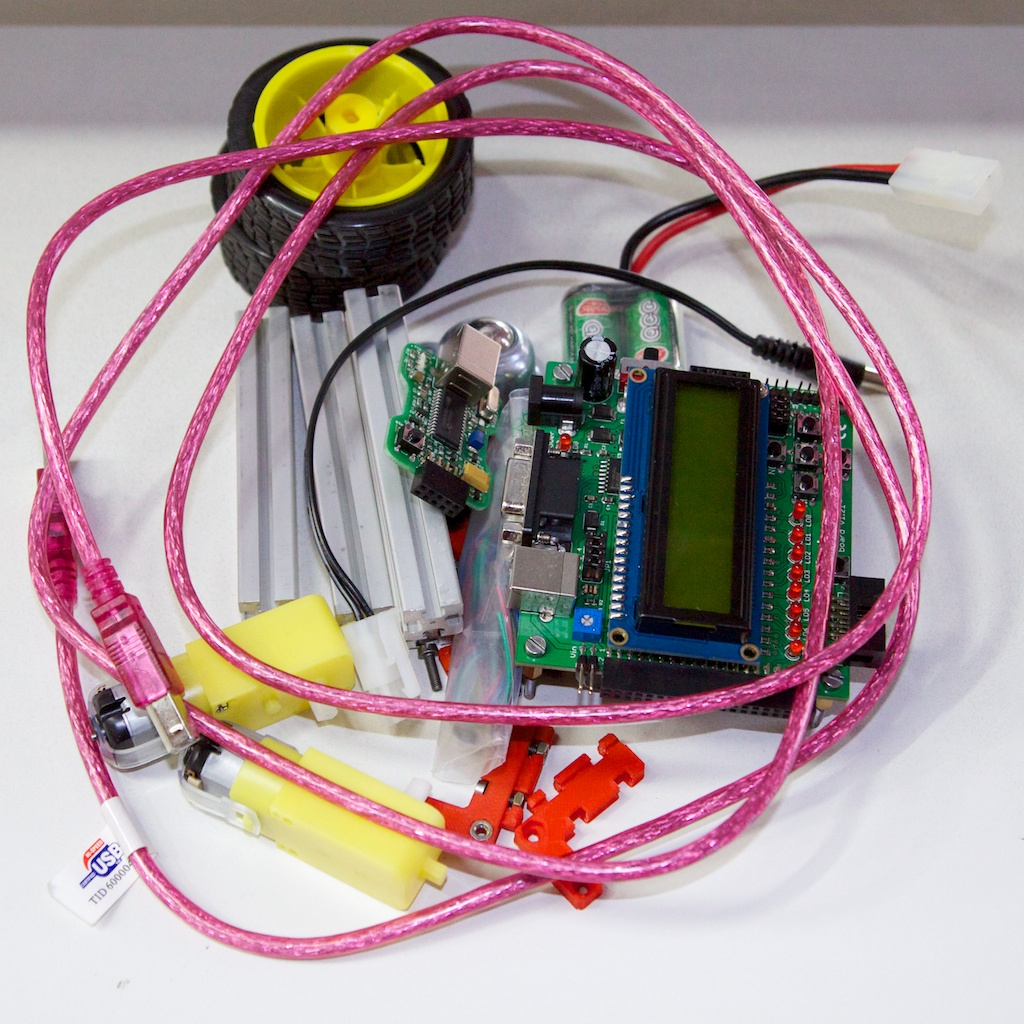
\includegraphics[width=0.5\textwidth]{img/robot_parts.jpg}\label{fig:parts}
\caption[]{Parts}
\end{center}
\end{figure}

\section{Inquiry based robotics learning}
Details of the setup of the workshops itself, all pedagogical aspects.

\section{Robotics trick students into learning}
Robots build by the students, details of the google blockly results (for example, one student, aged 13 was able to complete all 10 mazes within xx minutes while others including teachers took 2 hours), feedback given by students and teachers and the scores given.

\begin{figure}[htp]
\subfigure[]{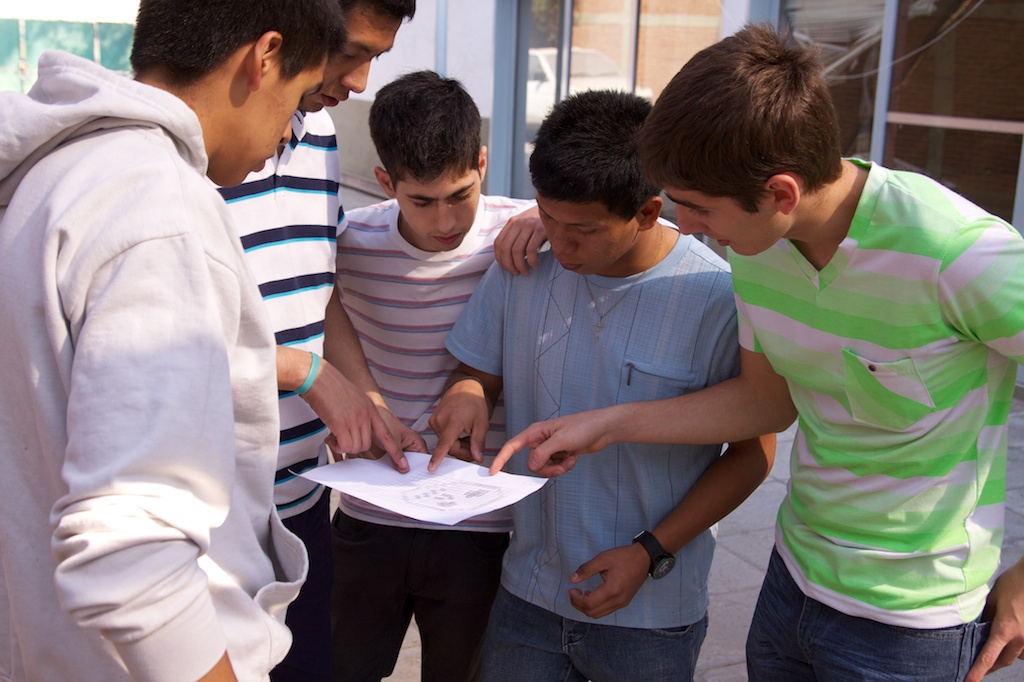
\includegraphics[width=0.325\textwidth]{img/cs_unplugged.jpg}\label{fig:cs_unplugged}}
\subfigure[]{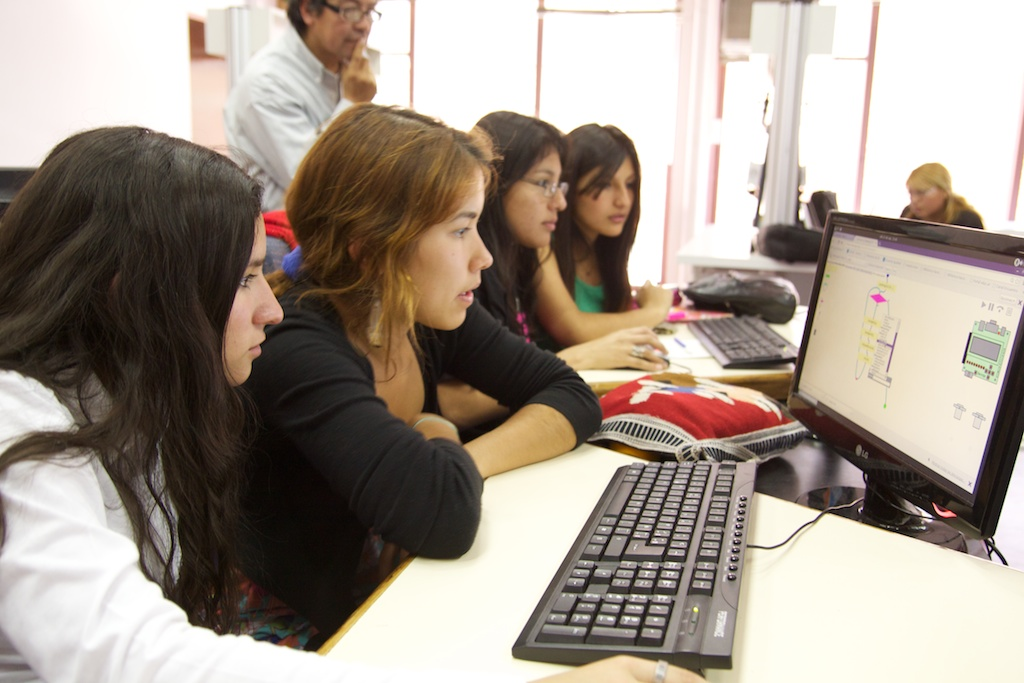
\includegraphics[width=0.325\textwidth]{img/programming.jpg}\label{fig:programming}}
\subfigure[]{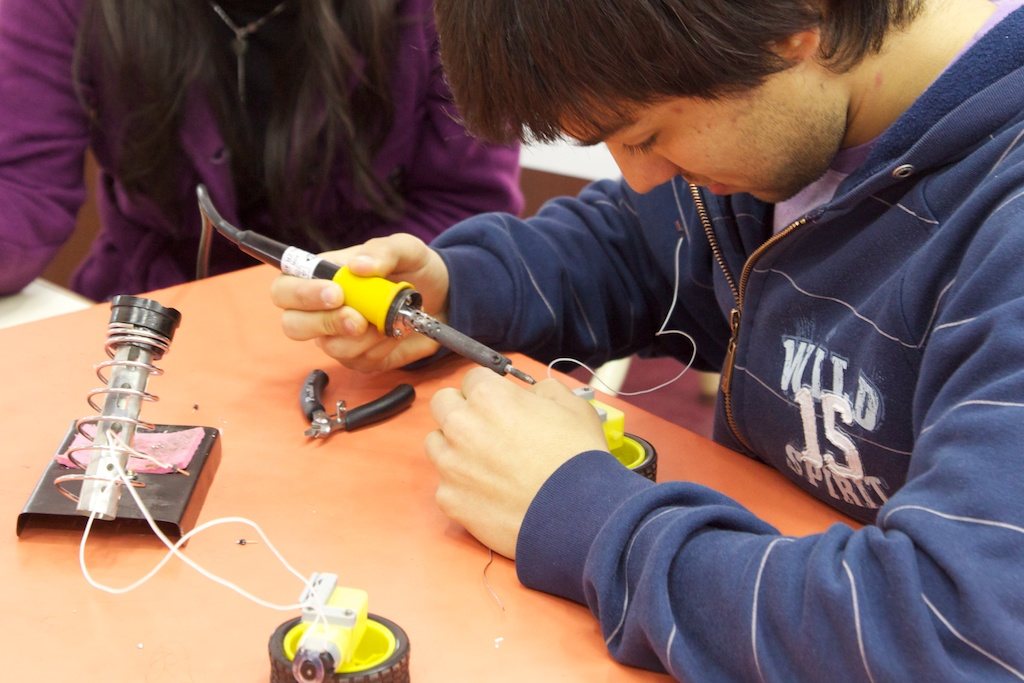
\includegraphics[width=0.325\textwidth]{img/robot_soldering.jpg}\label{fig:soldering}}
\subfigure[]{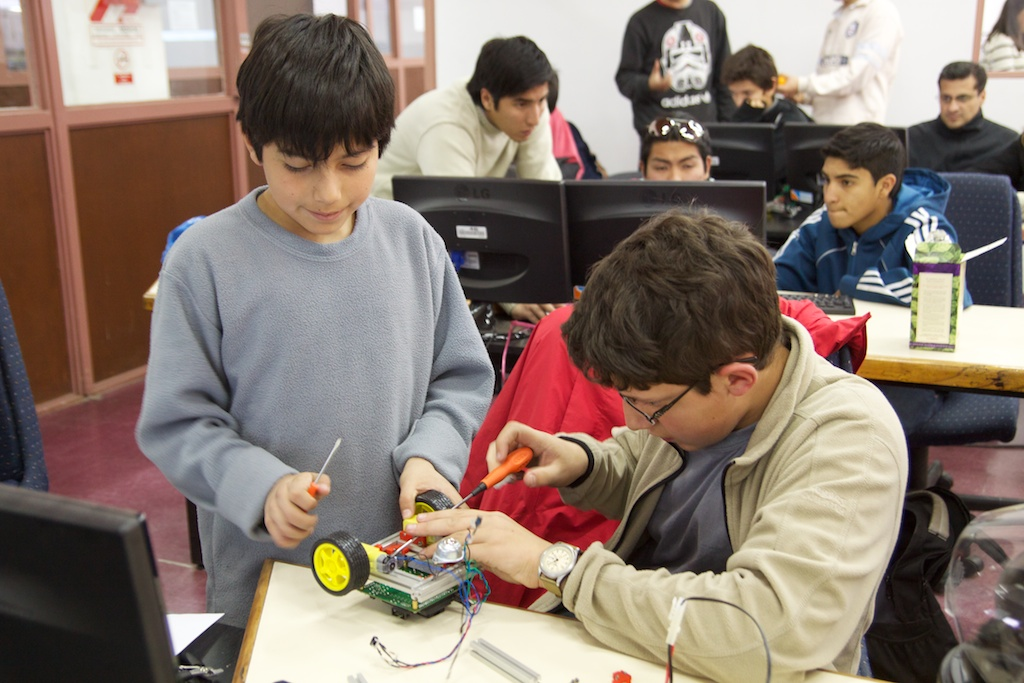
\includegraphics[width=0.325\textwidth]{img/robot_building_a.jpg}\label{fig:building_a}}
\subfigure[]{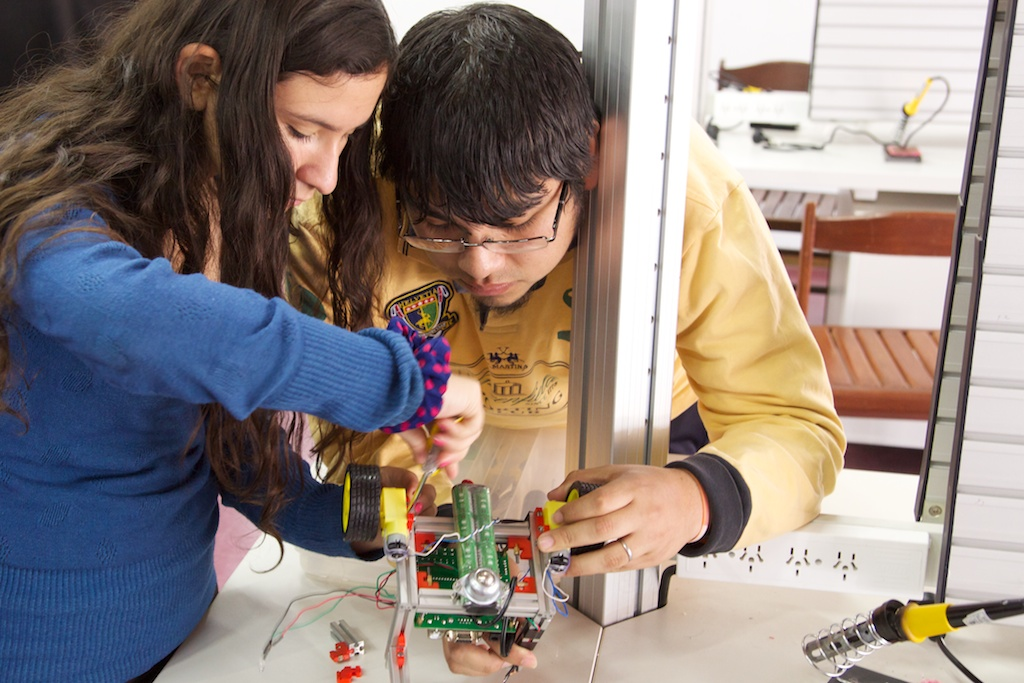
\includegraphics[width=0.325\textwidth]{img/robot_building_b.jpg}\label{fig:building_b}}
\subfigure[]{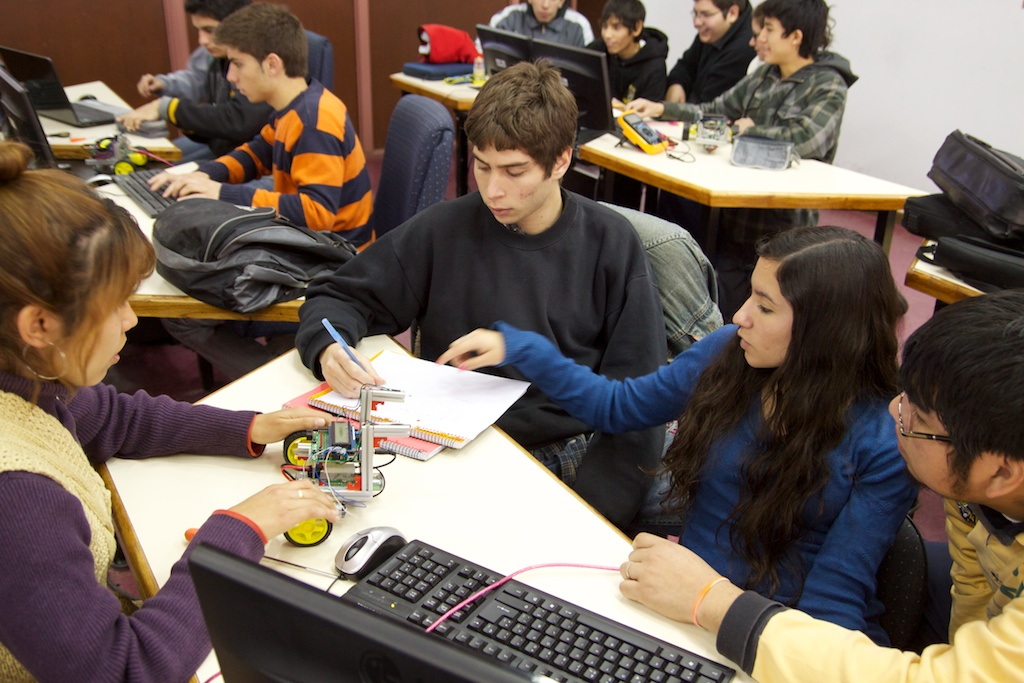
\includegraphics[width=0.325\textwidth]{img/robot_programming.jpg}\label{fig:robot_programming}}
\subfigure[]{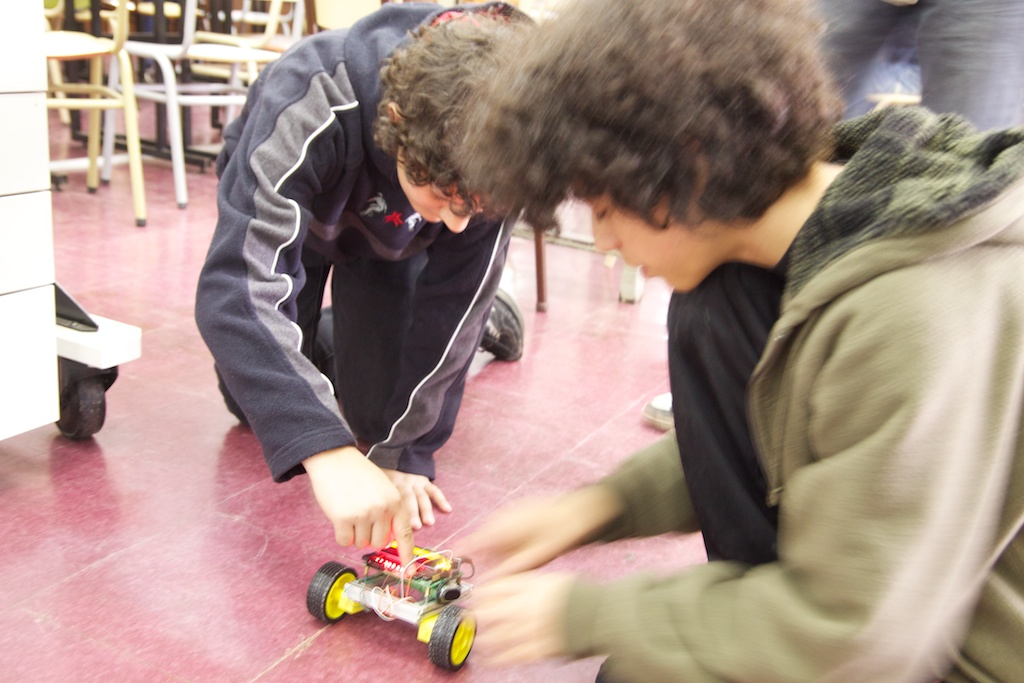
\includegraphics[width=0.325\textwidth]{img/robot_testing_a.jpg}\label{fig:robot_testing_a}}
\subfigure[]{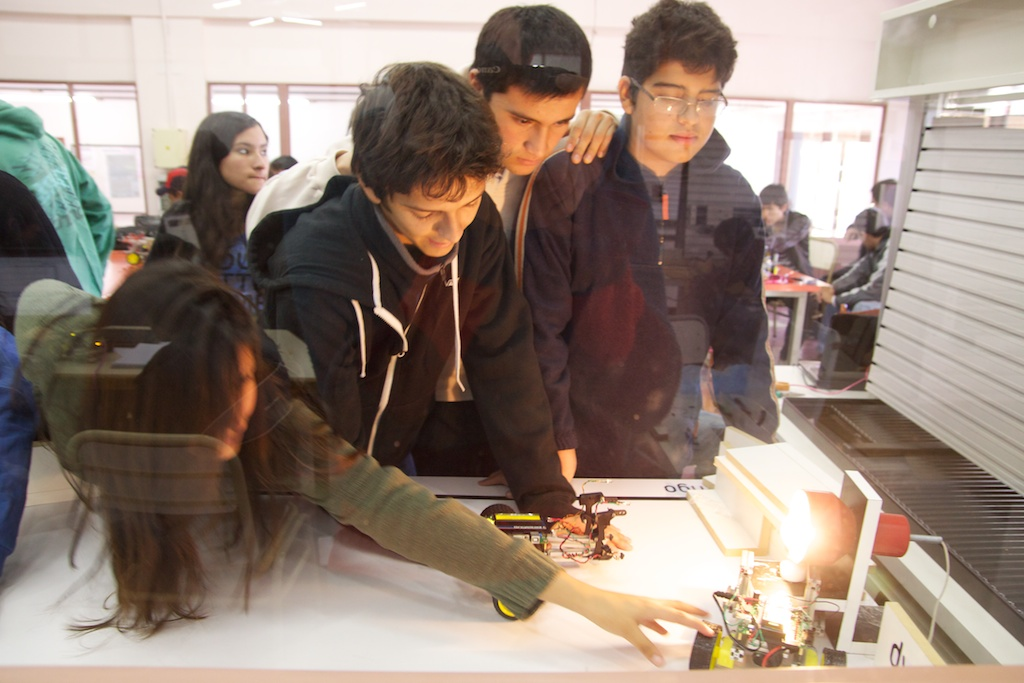
\includegraphics[width=0.325\textwidth]{img/robot_testing_b.jpg}\label{fig:robot_testing_b}}
\subfigure[]{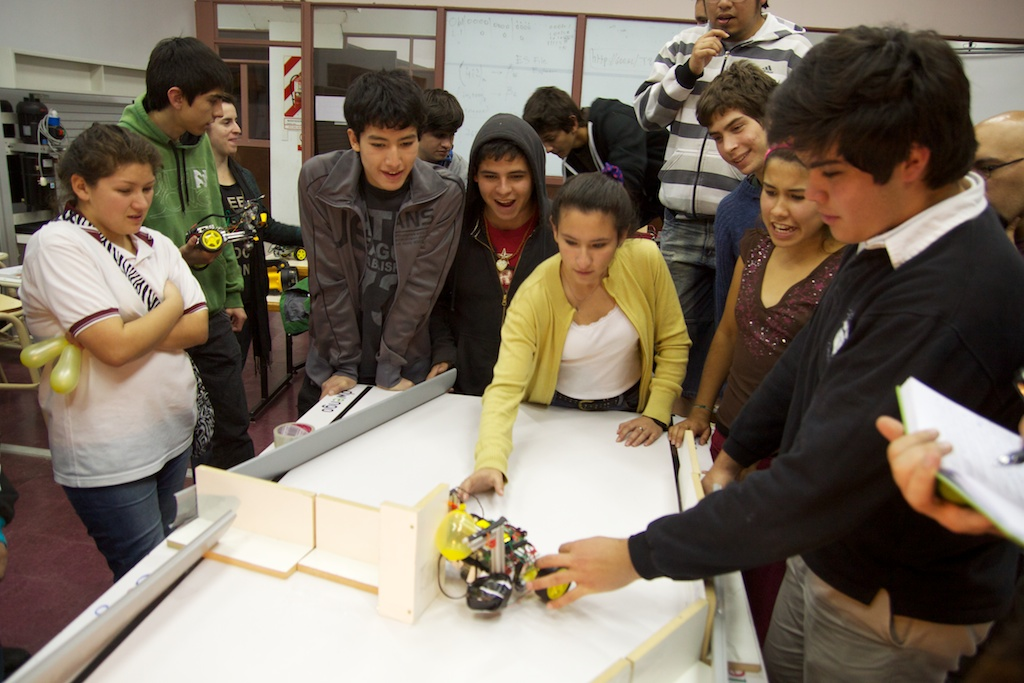
\includegraphics[width=0.325\textwidth]{img/competition.jpg}\label{fig:competition}}
\caption[]{Workshop overview.}
\end{figure}

\section{From a local project to international outreach}
Direct impact: amount of students and teachers we taught, parents that came and visited the competitions, media attention in Salta; Sustainability of the impact: local production of the Dwengo board, continuation of the project in the schools (driven by a careful selection of the teachers and continuous stimulation of them), and the outreach to other countries including Brazils and Bolivia? Chile?

\section{Conclusions}
Goals that we met, collaboration on an international level, decentralisation, spread of pedagogical ideas, technology and values.


%%%%%%%%%%%%%%%%%%%%%%%%%%%%%%%%%%%%%%%%%%%%%%%%%%%%%%%%%%%%%%%%%%%%%%%%%%%%%%%%
\section*{Acknowledgment}
The project presented in this paper was never possible without the unconditional support of the Dwengo volunteers, the newly designed building bricks for robots by Cesar Vandevelde of the Howest, the financial support by Google within the Google RISE framework, the corporation of Dra. Mar\'ia Soledad Vicente of Ministry of Education, Science and Technology of the Salta province, and the infrastructure and support of the U.F.I.De.T.

%%%%%%%%%%%%%%%%%%%%%%%%%%%%%%%%%%%%%%%%%%%%%%%%%%%%%%%%%%%%%%%%%%%%%%%%%%%%%%%%
\bibliographystyle{IEEEtran}
\bibliography{trtwr2014}

\end{document}
